\begin{frame}{Modelo Discriminador}
    
    \begin{block}{Modelo}
        La salida de este modelo es una probabilidad de que la imagen del modelo generador sea tomada
        como una real y a partir de esto clasificarla como un 1 o u 0 (Clasificador Binario) es por esto que nuestra salida es una función 
        \emph{Sigmoide}, ya que abarca valores de 0 a 1.
    \end{block}  
    \begin{figure}[H]
        \begin{center}
          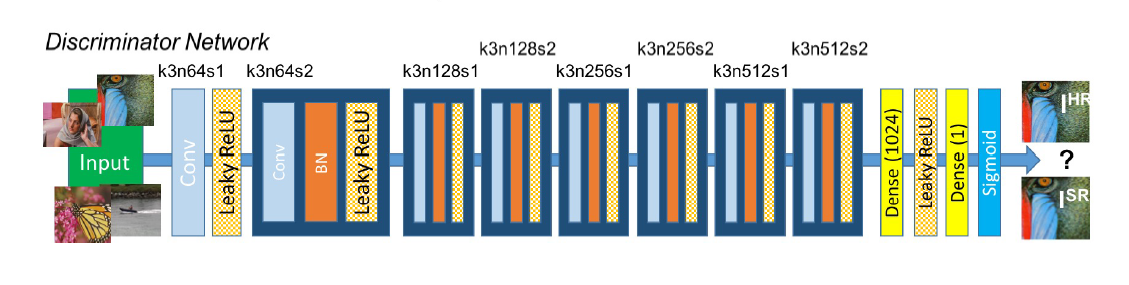
\includegraphics[scale = 0.5]{Imp_discriminador.png}
          \caption{Modelo de entrenamiento del discriminador}
          \label{Alexis3}
        \end{center}
    \end{figure}
     

\end{frame}

\begin{frame}{Modelo Generador}
    
    \begin{block}{Modelo}
        En este modelo la entrada es un vector de ruido aleatorio\emph{(z)} se da como señal de entrada 
        y se espera una imagen falsa como salida, esta imagen deberá aproximarse a la real.
    \end{block} 
        
    \begin{figure}[H]
        \begin{center}
          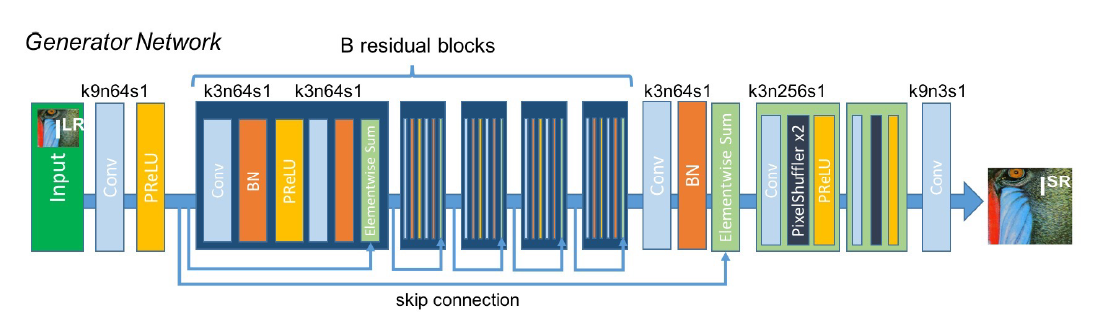
\includegraphics[scale = 0.5]{Imp_generador.png}
          \caption{Modelo de entrenamiento del generador}
          \label{Alexis4}
        \end{center}
    \end{figure}
     

\end{frame}



\begin{frame}{Redes residuales}
    \begin{block}{Bloque Residual}
        Realizan la conexión entre capas anteriores con capas futuras (saltos) sin que la información de 
        las características extraídas en capas previas se diluya.
    \end{block}
    \begin{figure}[H]
        \begin{center}
          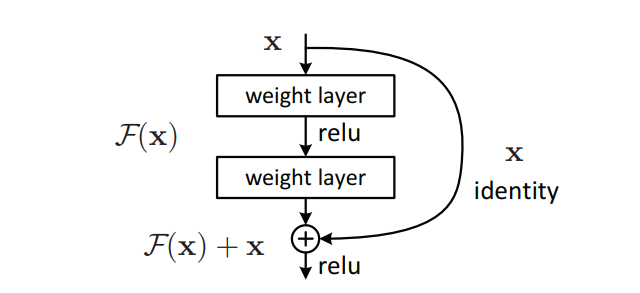
\includegraphics[scale = 0.2]{Residual-Block.png}
          \caption{Funcionamiento del Bloque Residual}
          \label{Alexis10}
        \end{center}
    \end{figure}

\end{frame}


\begin{frame}{Bloques de escalado}
    \begin{block}{Escalado}
        
        El bloque de upsampling es el que nos ayudara a realizar el escalado de la imagen conforme al entrenamiento,
        se encarga de realizar un aumento de pixeles mediante interpolaciones de vecino cercano para cada 
        capa de convolución lo que se interpreta en un suavizado de la imagen y así mismo un aumento de tamaño.
    \end{block}
    \begin{figure}[H]
        \begin{center}
          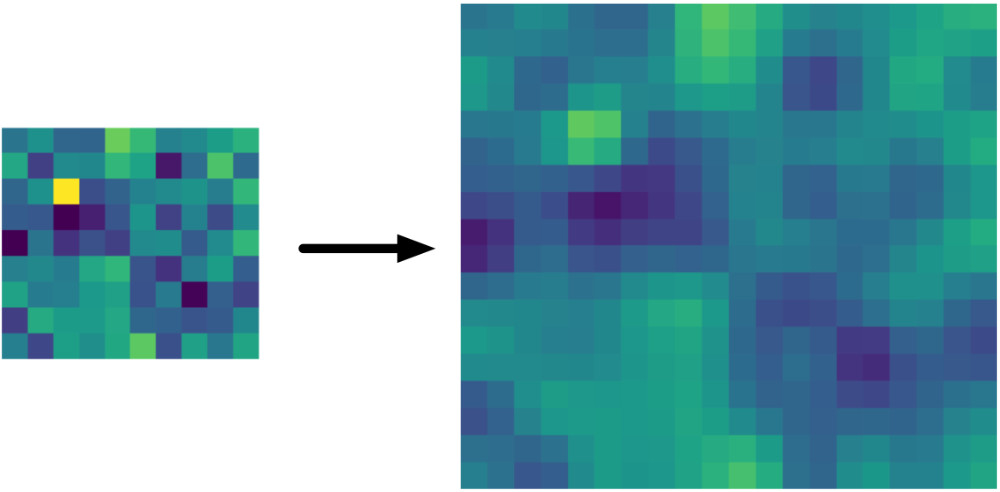
\includegraphics[scale = 0.6]{Bilinear2x.jpg}
          \caption{Escalado de la imagen de entrada}
          \label{Alexis11}
        \end{center}
    \end{figure}
     
\end{frame}

\begin{frame}{VGG19}
    
\begin{block}{Red Pre-entrenada}
    VGG19 (Visual Geometry Group) es la red convolucional pre-entrenado que se utiliza en el código,
    dedicada a la clasificación de imágenes ,consta de 16 capas convolucionales.
\end{block}
    \begin{figure}[H]
        \begin{center}
          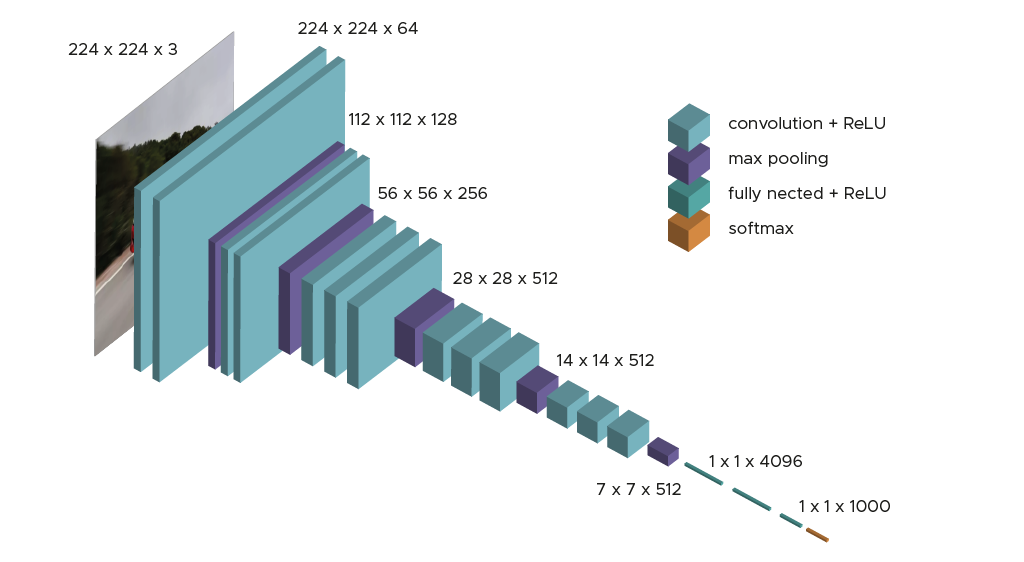
\includegraphics[scale = 0.18]{VGG19.png}
          \caption{Red Neuronal Pre-entrenada}
          \label{Alexis12}
        \end{center}
    \end{figure}
     

\end{frame}

\begin{frame}{Binary Crossentropy}
\begin{block}{Binary Crossentropy}
    Con esta función se logra realizar la clasificación de probabilidades del discriminador
    (0 a 1) y castiga al modelo en caso de que exista un dato catalogado erróneo.
\end{block}
    \begin{figure}[H]
        \begin{center}
          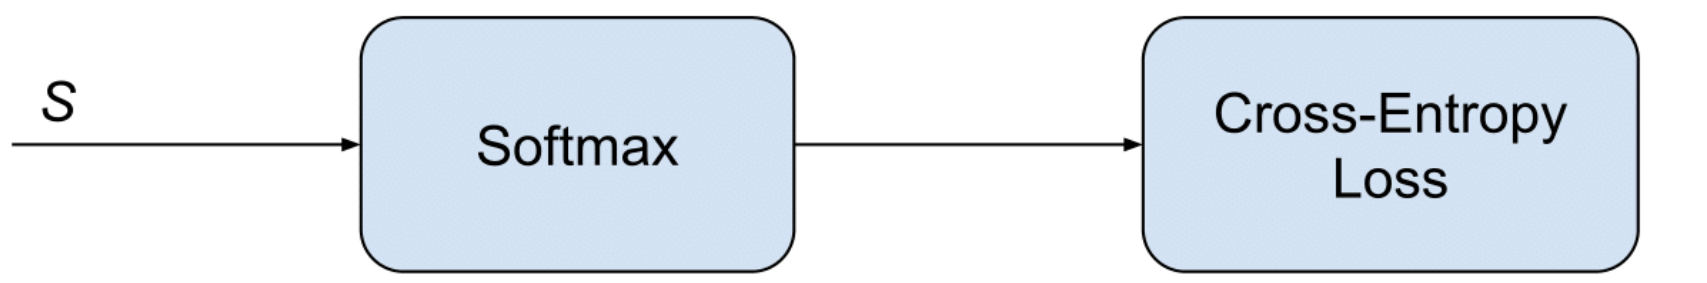
\includegraphics[scale = 0.18]{binarycross.png}
          \caption{Función binaria}
          \label{Alexis12}
        \end{center}
    \end{figure}
     

\end{frame}

\begin{frame}{Modelos Generadores obtenidos}
    \begin{block}{Modelo del entrenamiento.}
        Se obtiene un archivo comprimido, con los datos del modelo generador en este caso.
    \end{block}
    \begin{figure}[H]
        \begin{center}
          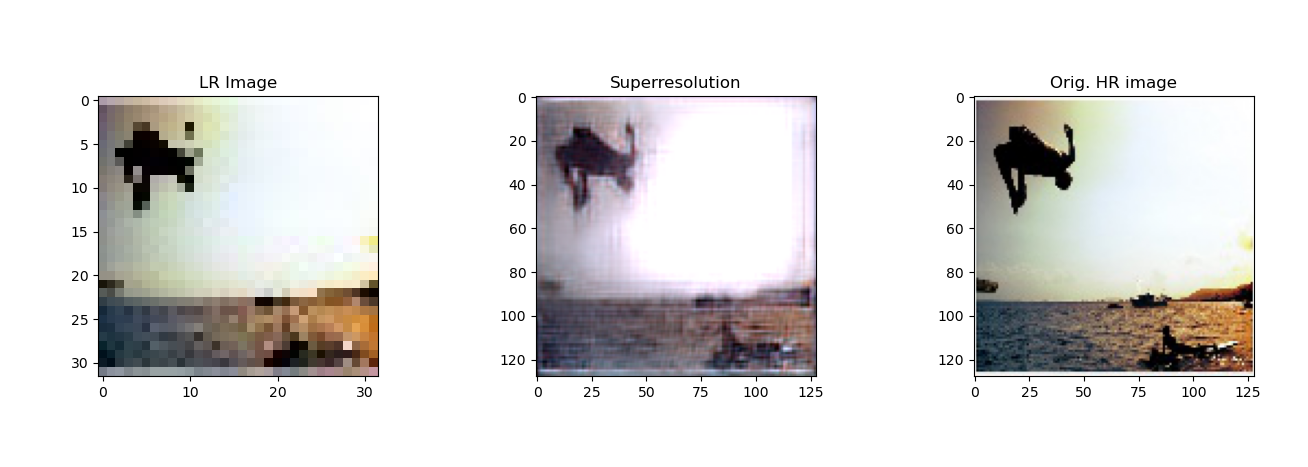
\includegraphics[scale = 0.6]{13im_200E.png}
          \caption{Modelo de entrenamiento del generador}
          \label{Alexis6}
        \end{center}
    \end{figure}
    
\end{frame}

\begin{frame}{Modelos Generadores obtenidos}
  
    \begin{figure}[H]
        \begin{center}
          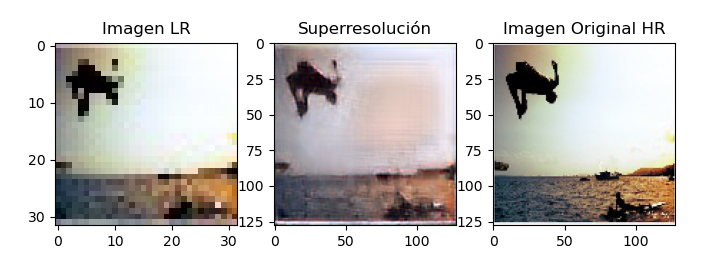
\includegraphics[scale = 0.6]{50im_400E.png}
          \caption{Modelo entrenado con 50 imágenes y 400 épocas}
          \label{Alexis7}
        \end{center}
    \end{figure}
     
\end{frame}


\begin{frame}{Modelos Generadores obtenidos}
    \begin{block}{Re-entrenamiento}
        Se puede cargar una configuración del modelo generador anterior, esto disminuye las pérdidas 
        debido a los pesos y criterio del entrenamiento.
    \end{block}
    \begin{figure}[H]
        \begin{center}
          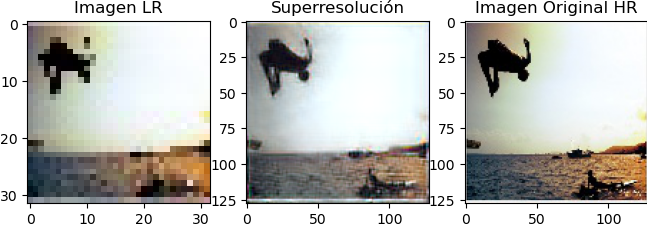
\includegraphics[scale = 0.6]{1000im_5E_Reentrenado.png}
          \caption{Modelo reentrenado 1000 imágenes, 5 épocas}
          \label{Alexis8}
        \end{center}
    \end{figure}
     
\end{frame}


\begin{frame}{Pérdidas del modelo}
    \begin{block}{Función de pérdida}
        
   
        Como parte del entrenamiento se necesitan parámetros que nos describan de manera correcta los resultados
        que obtenemos de la predicción en nuestra red neuronal, para esto se hace el uso de funciones de perdida, estas funciones 
        evalúan la desviación entre las predicciones realizadas por la red neuronal y los valores 
        reales de las observaciones utilizadas durante el aprendizaje.
        
        Cuanto menor es el resultado de esta función, 
        más eficiente es la red neuronal.

    \end{block}    
\end{frame}

\begin{frame}{Pérdidas del modelo}
    
    \begin{figure}[H]
        \begin{center}
          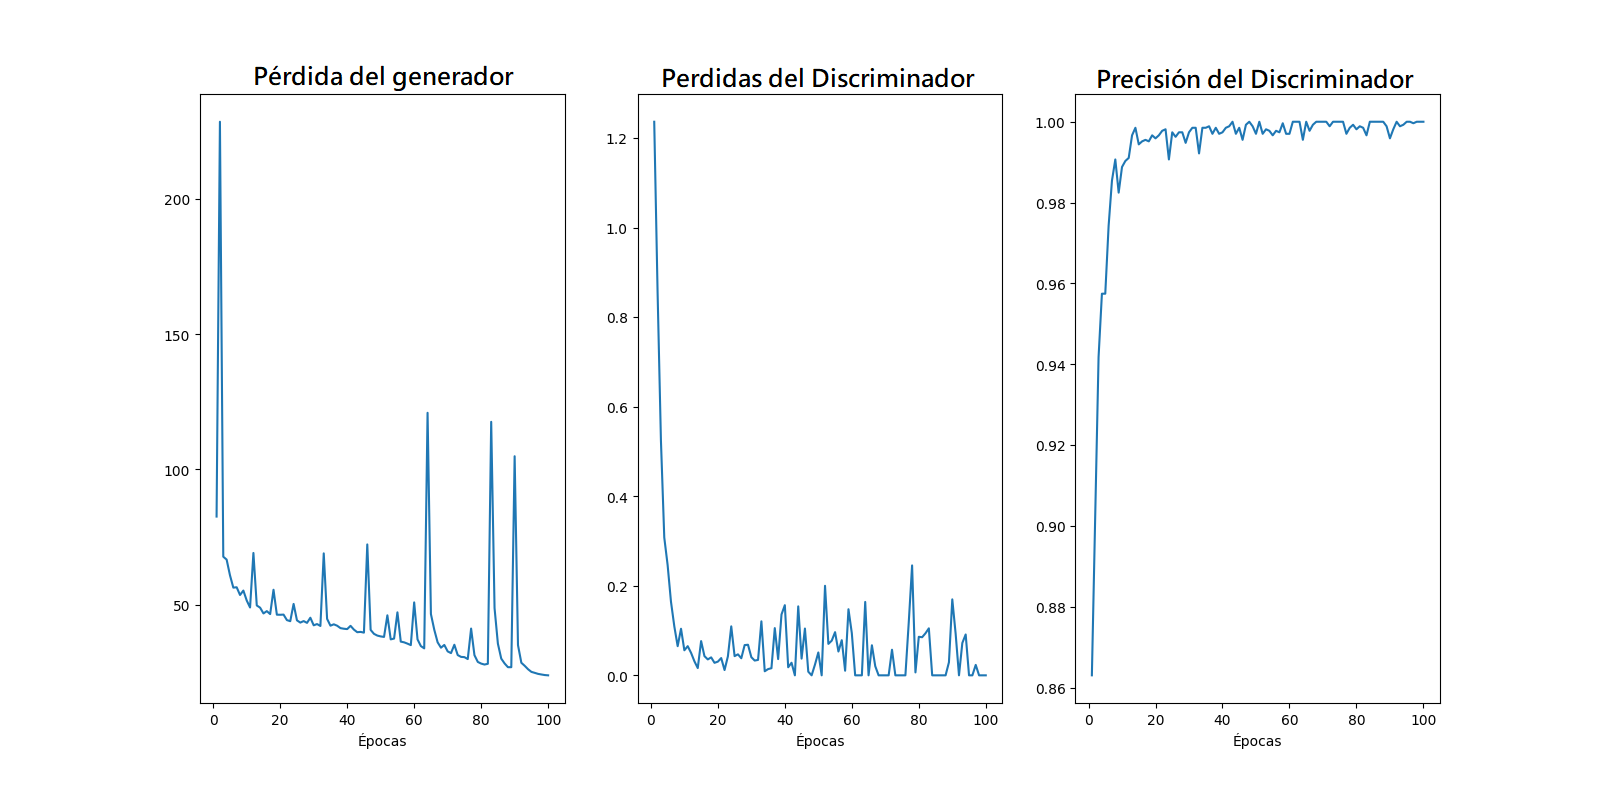
\includegraphics[scale = 0.4]{Graficasperdidas.png}
          \caption{Pérdidas y Precisión del Modelo}
          \label{Alexis13}
        \end{center}
    \end{figure}
     
\end{frame}


